\documentclass[12pt]{article}
\usepackage[utf8]{inputenc}
\usepackage{amsmath}
\usepackage{systeme}
\usepackage{amsfonts}
\usepackage{graphicx}
\usepackage{enumitem}
\usepackage{hyperref}
\usepackage{xcolor}
\usepackage{kbordermatrix}
\usepackage{centernot}
\usepackage{xcolor}

\title{%
	\textbf{Notițe Seminar 8}}

\begin{document}
	
	\maketitle
	
	\textbf{{Intro:}} Seminarul acesta vom continua cu un alt algoritm de clasificare. Vom vedea că el poate fi folosit și pentru regresie. Va fi ultimul algoritm de clasificare pe care îl vom studia. De săptămâna viitoare vom trece la învățare nesupervizată de tip clusterizare.

	\section{Remember}
	\subsection{Vectori}
	
	Vom lucra cu \textbf{vectori} din $\mathbb{R}^n$, care sunt niște tuple de numere reale: $(x_1,\dots,x_n) \in \mathbb{R}^n$. Noi vom folosi notația prin care un vector va fi o matrice cu o singură coloană: $\begin{bmatrix}
	x_1\\
	\vdots\\
	x_n
	\end{bmatrix} \in \mathbb{R}^n$.

	\subsection{Distanțe}
	
	Dacă vă interesează definiția, vedeți ex. 2/pag. 427.
	
	O familie de distanțe este dată de distanța Minkowski (sau distanța indusă de norma $p$):
	
	$$d_p\left( \begin{bmatrix}
	x_1\\
	\vdots\\
	x_n
	\end{bmatrix}, \begin{bmatrix}
	y_1\\
	\vdots\\
	v_n
	\end{bmatrix} \right) = \left( |x_1 - y_1|^p + \dots + |x_n - y_n|^p \right)^\frac{1}{p},$$
	unde $p \geq 1$.
	
	Pentru $p=1$ obținem distanța Manhattan (\textit{taxicab/city block}). Exemplu:
	$$d_1\left( \begin{bmatrix}
	1\\
	2
	\end{bmatrix}, \begin{bmatrix}
	3\\
	5
	\end{bmatrix} \right) = |1 - 3| + |2 - 5| = 5$$
\begin{center}
	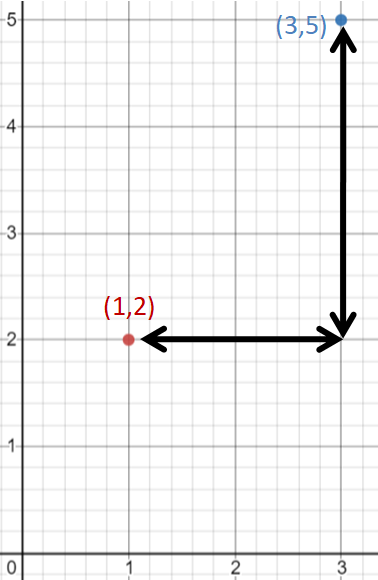
\includegraphics{screenshot001}
\end{center}


	Pentru $p=2$ obținem \textbf{distanța euclidiană}. Exemplu:
	$$d_2 \left( \begin{bmatrix}
		1\\
		2
		\end{bmatrix}, \begin{bmatrix}
		3\\
		5
		\end{bmatrix} \right) = d \left( \begin{bmatrix}
		1\\
		2
		\end{bmatrix}, \begin{bmatrix}
		3\\
		5
		\end{bmatrix} \right) = \sqrt{(1-3)^2 + (2-5)^2} = \sqrt{2^2 + 3^2} = \sqrt{13}$$
	
	\begin{center}
		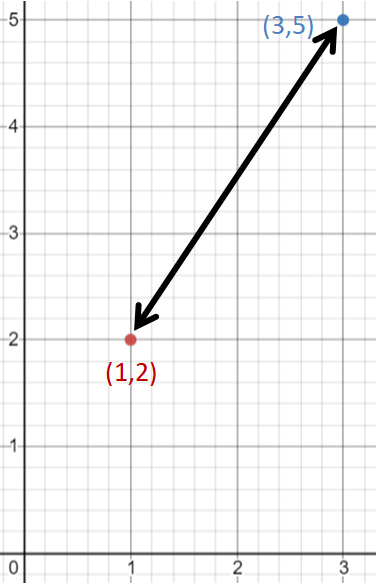
\includegraphics{screenshot002}
	\end{center}
	
	
	\textbf{Implicit}, dacă într-un exercițiu nu se specifică cu ce distanță se lucrează, atunci se va lucra cu distanța euclidiană.
	
	
	Pentru $p=\infty$ obținem distanța Cebîșev. Exemplu:
	$$d_\infty \left( \begin{bmatrix}
	1\\
	2
	\end{bmatrix}, \begin{bmatrix}
	3\\
	5
	\end{bmatrix} \right) = \max \{|1-3|,|2-5|\} = \max \{2,3\} = 3$$
	
	\begin{center}
		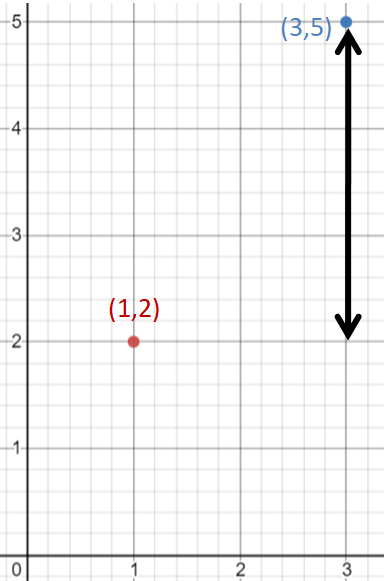
\includegraphics{screenshot003}
	\end{center}
	
	
	Nu trebuie să rețineți numele distanțelor, ci doar să aplicați o distanță în funcție de $p$.
	
	\section{kNN = k Nearest Neighbours}
	
	 - $k$ este un număr natural nenul pe care îl setăm înainte de a aplica algoritmul.
	
	- suntem tot în contextul învățării supervizate de tip clasificare, dar vom putea face și regresie
	
	- totuși, până acum am fost în cazul în care algoritmii făceau ceva la antrenare (ID3 făcea un arbore; AB făcea funcția/ansamblul $H_T(x)$; NB și JB făceau niște estimări de probabilități/parametri); kNN nu face mai nimic la antrenare: doar memorează datele (de aici vine și titlul capitolului din carte: \textit{Învățare bazată pe memorare}); abia la testare, când vine o instanță își creează modelul și furnizează eticheta prezisă; astfel, despre kNN se va spune că este \textbf{\textit{lazy}} și despre ID3, AB, NB, JB, că sunt \textbf{\textit{eager}}.
	
	\begin{center}
		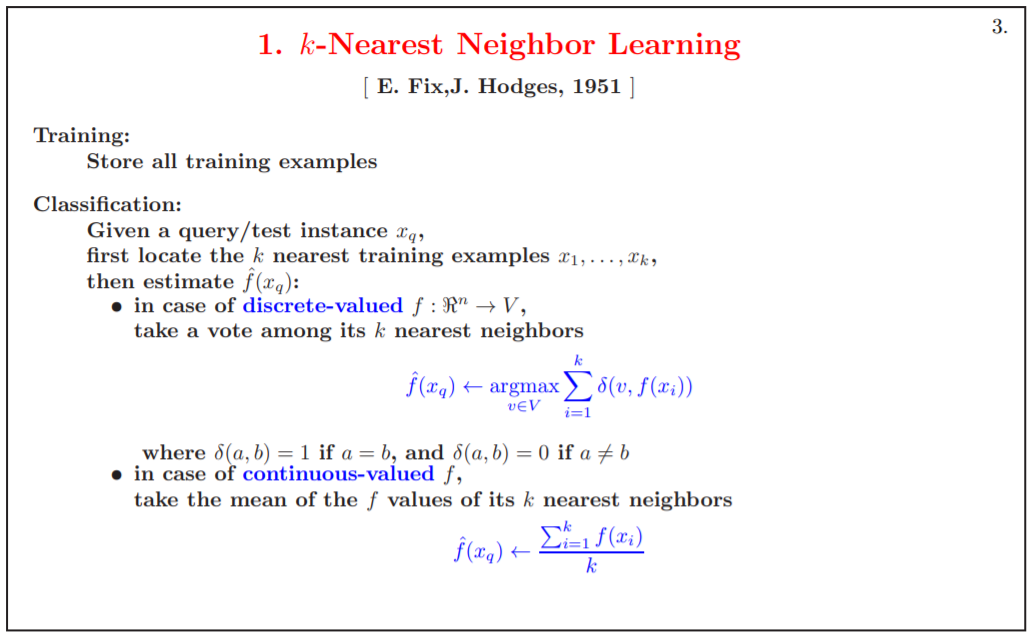
\includegraphics[width=1\linewidth]{screenshot004}
	\end{center}
	\begin{center}
		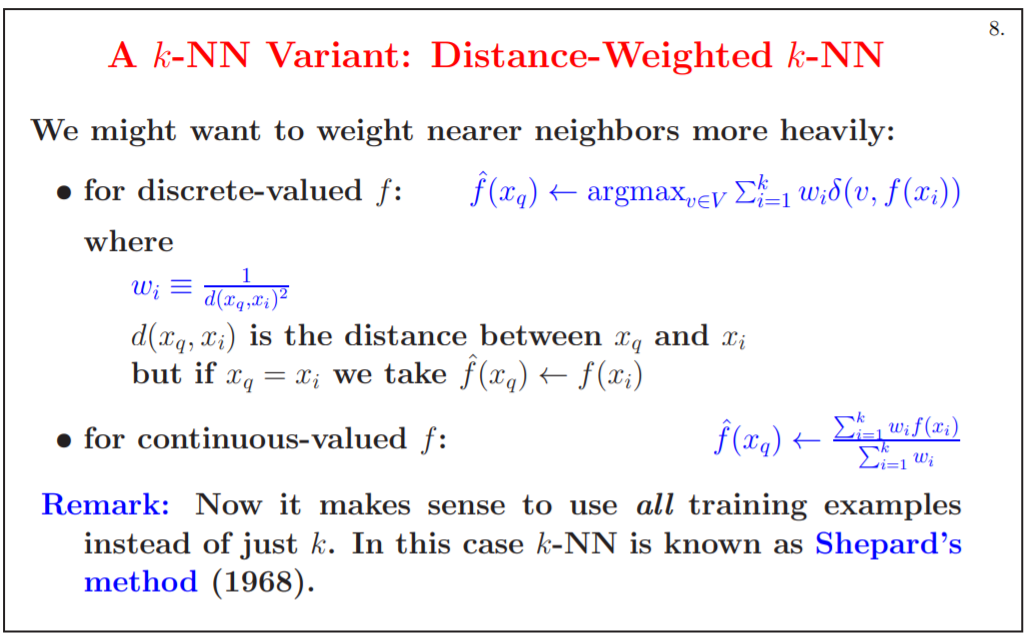
\includegraphics[width=1\linewidth]{screenshot005}
	\end{center}
	(slide-uri preluate din \url{https://profs.info.uaic.ro/~ciortuz/SLIDES/ml8.pdf})
	
\textbf{	Aplicare 3NN (kNN când $k=3$):}
	
	Date de antrenare: A, B, C, D (etichetele sunt date în imagini)
	
	Date de test: Z
	
	3NN vecinătatea lui Z (adică cei mai apropiați 3 vecini ai lui Z, adică cele mai apropiate 3 puncte de Z) este $\{A,B,C\}$.
	
	Observație: pentru a afla kNN vecinătatea nu trebuie neapărat să calculați distanțe, ci puteți să desenați niște cercuri pe desen. De exemplu, vedeți ex. 1/pag. 426.
	
	\begin{enumerate}
		\item \textbf{Clasificare} (prezice o clasă/\textit{ceva discret})
		\begin{center}
			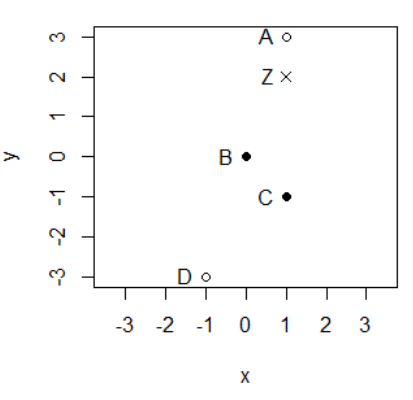
\includegraphics{screenshot006}
		\end{center}
		\begin{enumerate}
			\item \textbf{fără ponderi}
			
			Pentru $\circ$ vom avea un singur vot: de la A.
			
			Pentru $\bullet$ vom avea 2 voturi: de la B și C.
			
			$$
			\left.
			\begin{array}{ll}
			\circ: 1 \\
			\bullet: 2
			\end{array}
			\right \} \stackrel{\text{argmax}}{\Rightarrow} \bullet
			$$
			Deci, returnăm $\bullet$ pentru Z.
			
			Observație: Când lumea vorbește despre kNN, de obicei, se referă la aest caz: clasificare, fără ponderi.
			
			\item \textbf{cu ponderi}
			
			Voturile de mai înainte vor fi înlocuite cu ponderi. Ponderile sunt construite în așa fel încât o pondere mare corespunde unui punct apropiat, iar o pondere mică, unui punct îndepărtat. Dacă nu se specifică atfel în enunț, veți folosi ponderile din slide-uri de mai sus (și distanța euclidiană).
			
			$$
			\left.
			\begin{array}{ll}
			\circ: w_A = \frac{1}{d^2(A,Z)} = \frac{1}{1} = 1 \\
			\bullet: w_B + w_C = \frac{1}{d^2(B,Z)} + \frac{1}{d^2(C,Z)} = \frac{1}{\sqrt{1^2 + 2^2}^2} + \frac{1}{\sqrt{3^2}^2} =  \frac{1}{5} + \frac{1}{9} = 0.3111
			\end{array}
			\right \} \stackrel{\text{argmax}}{\Rightarrow} \circ
			$$
			Deci, returnăm $\circ$ pentru Z.
			
			Observație: eticheta furnizată pentru Z de către kNN cu ponderi a ieșit diferită de eticheta dată de kNN fără ponderi.
		\end{enumerate}
		\item \textbf{Regresie} (prezice un număr real/\textit{ceva continuu})
		\begin{center}
			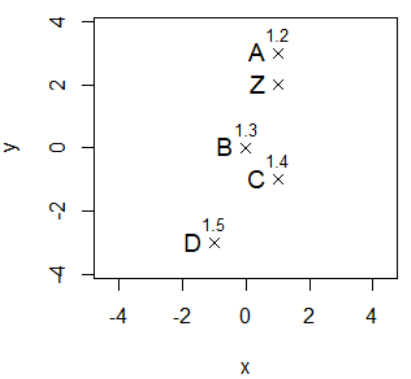
\includegraphics{screenshot007}
		\end{center}
	\newpage
		\begin{enumerate}
			\item \textbf{fără ponderi}
			
				Pentru Z vom returna media aritmetică a etichetelor pentru A, B, C:
				$$\frac{1.2+1.3+1.4}{3} = 1.3$$
			\item \textbf{cu ponderi}
			
				Pentru Z vom returna media aritmetică ponderată a etichetelor pentru A, B, C:
				$$\frac{w_A \cdot 1.2 + w_B \cdot 1.3 + w_C \cdot 1.4}{w_A + w_B + w_C} = \frac{\frac{1}{d^2(A,Z)} \cdot 1.2 + \frac{1}{d^2(B,Z)} \cdot 1.3 + \frac{1}{d^2(C,Z)} \cdot 1.4}{\frac{1}{d^2(A,Z)} + \frac{1}{d^2(B,Z)} + \frac{1}{d^2(C,Z)}} =$$
				$$= \frac{1 \cdot 1.2 + 0.2 \cdot 1.3 + 0.1111 \cdot 1.4}{1 + 0.2 + 0.1111} = 1.2322$$
		\end{enumerate} 
	\end{enumerate}
	
	Algoritmul lui \textbf{Shepard}: Cazul 2b de mai sus, DAR impunem $k$ să fie egal cu numărul de instanțe din setul de antrenament, adică, pe exemplul anterior, avem că eticheta furnizată pentru Z va fi:
	$$\frac{w_A \cdot 1.2 + w_B \cdot 1.3 + w_C \cdot 1.4 + w_D \cdot 1.5}{w_A + w_B + w_C + w_D} = \dots$$
	
		De obicei, ar trebui \textbf{să se specifice 3 chestiuni înainte de aplicarea lui kNN}:
	\begin{itemize}
		\item $k$
		\item distanța folosită; dacă nu se specifică, atunci folosiți distanța euclidiană, după cum am mai zis
		\item 1 sau 2 euristici/convenții:
		\begin{itemize}
			\item ce se întâmplă dacă pentru al $k$-lea vecin avem mai mulți candidați aflați la aceeași distanță?
			\item \textit{doar dacă e cazul}: ce se întâmplă în caz de paritate de voturi
		\end{itemize}
	\end{itemize}
	
	- $k$ poate fi par, deși nu se recomandă să luam $k$ par pentru că trebuie să spunem ce se întâmplă în caz de paritate de voturi; 
	
	- chiar dacă $k$ este un număr par, putem avea un caz în care avem paritate de voturi; prima euristică poate crea acest caz
	
	\textbf{Atenție!} Calculați eroarea la antrenare și eroarea la CVLOO pentru datele din desen \textbf{pentru 1NN}:
	\begin{center}
		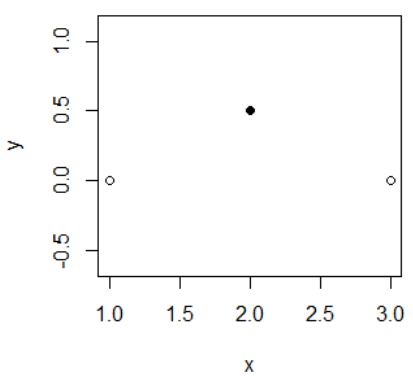
\includegraphics{screenshot008}
	\end{center}
	
	Eroarea la antrenare = 0 (cel mai apropiat vecin al unui punct este chiar acel punct)
	
	Eroarea la CVLOO = $\frac{3}{3}$ = 1
	
	În general: \textbf{Eroarea la antrenare pentru 1NN (folosind orice distanță) pentru date consistente este 0.}
	
	\subsection{Granițe de decizie pentru 1NN cu distanța euclidiană}
	
	Varianta 1: cea din carte, urmărind exercițiile rezolvate din carte unde se desenează granițele de decizie (vezi, spre exemplu, ex. 11a/pag. 447)
	
	Varianta 2: urmărind algoritmul descris mai jos. De menționat este că algoritmul nu este descris foarte în detaliu. Sper totuși că vă prindeți de ceea ce am vrut să vă zic prin el.
	\newpage
	\textbf{Algoritm pentru desenarea granițelor de decizie 1NN cu distanța euclidiană în 2 dimensiuni}
	
	\begin{enumerate}
		\item start
		\begin{enumerate}
			\item ne uităm la înfășurătoarea convexă a punctelor
			\item există segment pe ea cu vârfurile etichetate diferit?
			\begin{itemize}
				\item DA: de acolo începem
				\item NU: luăm un triunghi cu o latură cu vârfurile etichetate diferit astfel încât interiorul cercului circumscris să nu aibă vreun alt punct
			\end{itemize}
		\end{enumerate}
	 	\item Având o latură cu vârfurile etichetate diferit căutăm \textit{"cel mai apropiat"} punct, adică un punct astfel încât triunghiul format să nu includă alte puncte
	 	\item Ducem semi-mediatoarele în triunghiul respectiv
	 	\item Verificăm, având deja centrul cercului circumscris (de la 3)), dacă interiorul cercului circumscris triunghiului conține vreun punct (cu compasul)
	 	\begin{itemize}
	 		\item DA: revenim la 2), alegând alt punct și ștergând desenele de la 2) și 3)
	 		\item NU: atunci triunghiul este OK; mergem la pasul 5)
	 	\end{itemize}
 		\item Pe o altă latură a triunghiului cu vârfurile etichetate diferit:
 		\begin{itemize}
 			\item dacă latura aparține înfășurătorii convexe (\textit{"dă în afară"}): desenăm mediatoarea și \textit{în afară} și apoi revenim la pasul 1)
 			\item altfel: revenim la pasul 2)
 		\end{itemize}
	\end{enumerate}
	\textbf{Ne oprim}: când toate punctele etichetate diferit sunt separate.
	\newpage
	\textbf{Observații}:
	\begin{itemize}
		\item Dacă un punct se află pe un cerc, atunci punctul nu este considerat a fi în interiorul cercului.
		\item Triunghiurile OK care au fost alese pe parcurs nu trebuie să aibă vreo suprafață pe care să se suprapună.
		De exemplu:

		\begin{center}
			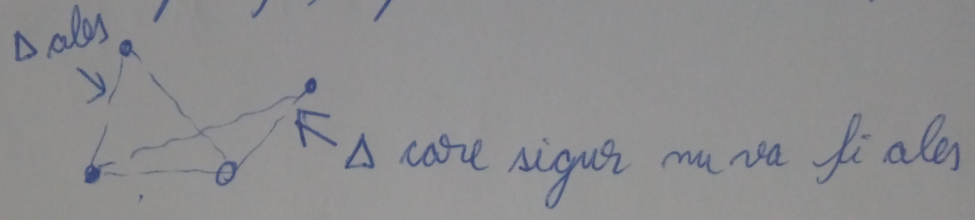
\includegraphics[width=1\linewidth]{screenshot009}
		\end{center}

		\item Pasul 1) ne dă o latură cu vârfurile etichetate diferit.
		\item Pașii 2)-4) ne dau un triunghi (cu semi-mediatoarele desenate).
		\item Pasul 5) ne spune cum continuăm.
		\item mediatoarea unui segment = perpendiculara pe segment ce conține mijlocul segmentului
		\item centrul cercului circumscris unui triunghi se află la intersecția mediatoarelor laturilor triunghiului.
	\end{itemize}
	
	\textbf{Exemple pentru pasul 3)}:
	
	(\textbf{Regula}: dinspre centru (centrul cercului circumscris/intersecția mediatoarelor) înspre \textit{"afara laturii"}))
	
	\begin{center}
		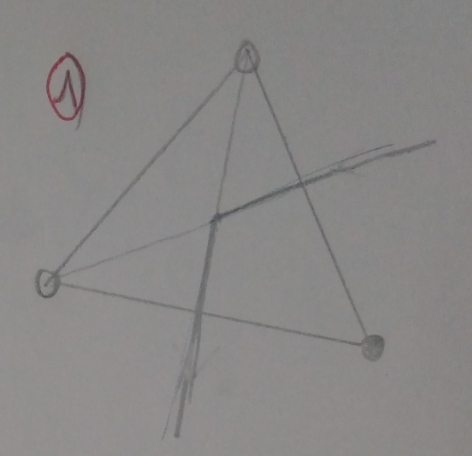
\includegraphics{screenshot010}
	\end{center}
	
	\begin{center}
		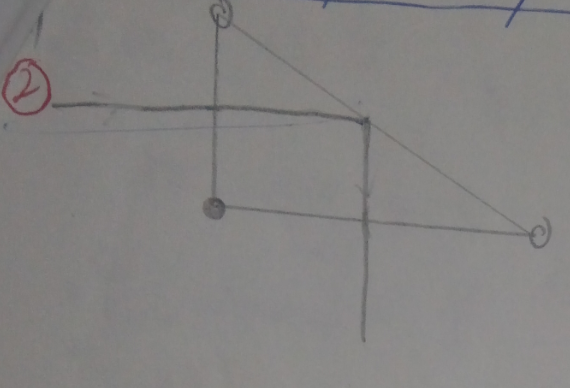
\includegraphics{screenshot011}
	\end{center}
	
	\begin{center}
		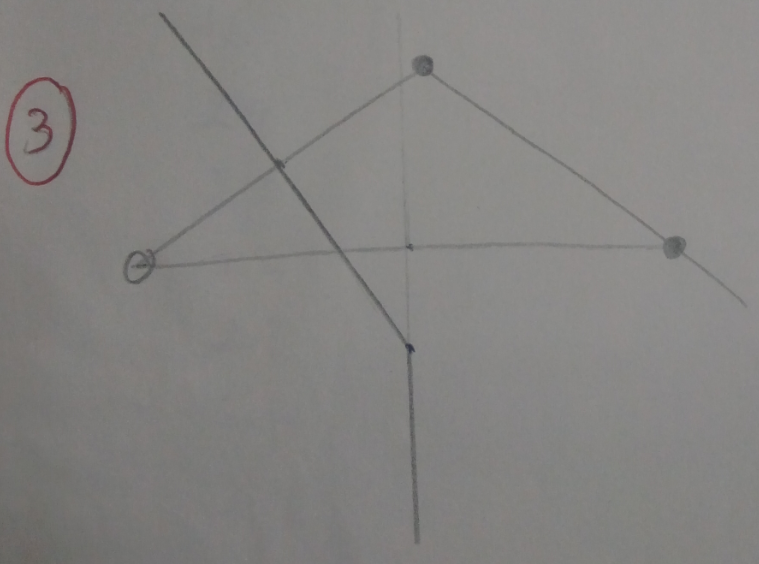
\includegraphics[width=0.7\linewidth]{screenshot012}
	\end{center}
	
	
	\newpage
	\textbf{\large{Schemă de final}}
	\begin{enumerate}
		\item Remember
		\begin{enumerate}
			\item Vectori
			\item Distanțe
		\end{enumerate}
		\item kNN
		\begin{enumerate}
			\item lazy vs eager
			\item
			\begin{enumerate}
				\item kNN pentru clasificare; fără ponderi
				\item kNN pentru clasificare; cu ponderi
				\item kNN pentru regresie; fără ponderi
				\item kNN pentru regresie; cu ponderi
				\item algoritmul lui Shepard
			\end{enumerate}
			\item 3 chestiuni de specificat înainte de aplicarea lui kNN
			\item eroarea la antrenare (pentru 1NN este zero dacă setul  de date este consistent)
			\item eroarea la CVLOO
			\item granițe de decizie pentru 1NN cu distanța euclidiană
		\end{enumerate}
	\end{enumerate}
	

	
\end{document}